%!TEX root = ../dissertation.tex
\begin{savequote}[75mm]
Nulla facilisi. In vel sem. Morbi id urna in diam dignissim feugiat. Proin molestie tortor eu velit. Aliquam erat volutpat. Nullam ultrices, diam tempus vulputate egestas, eros pede varius leo.
\qauthor{Quoteauthor Lastname}
\end{savequote}

\chapter{Related works}

\section{Phrase Grounding}

\subsection{Weakly Supervised Works}

Phrase grounding is the task that studies the mapping from noun
phrases to regions of an image (Sec.~\ref{sec:visual-grounding}) and
requires strong understanding of both visual and textual modalities,
specially when not all ground truth is available. 

Even if phrase grounding is an extremely relevant task, the study of
this problem in literature starts relatively late, mostly because a
community-accepted formalization of the problem took its time for
being developed. First efforts in this direction can be identified by
the work of S. Fidler \etal{} \cite{fidler2013sentence}. They
developed a model for semantic understanding of scene exploiting both
textual and visual information. In their work, short sentences are
parsed into nouns and prepositions, which are used to generate
potentials in a holistic scene model. An attempt to find an alignment
between entities in image and sentence is done by C. Kont \etal{}
\cite{kong2014you}. They proposed a model that exploits RGB-D images
(i.e., RGB images with depth channel) to detect the class of the 3D
objects, understand the scene type, and align the nouns/pronouns with
the referred visual objects. They used complex sentences, but
grounding is constrained to nouns of 21 object classes relevant to
indoor scenes. In the same period, R. Hu \etal{} \cite{hu2016natural}
moved to a slightly different task that requires to localize a target
object within a given image based on a natural language query of the
object, named natural language object retrieval. It differs from
text-based image retrieval task as it involves spatial information
about objects within the scene and global scene context. To address
this issue, they proposed a new model that scores proposals from
object retrieval by integrating information from contextual, spatial
and global features by means of a recurrent neural network. The advent
of Flickr30k Entities dataset collected and processed by B. Plummer
\etal{} \cite{plummer2015flickr30k} (described in
Sec.~\ref{subsec:flickr30k}) boosted the development of morea accurate
and general models, and allowed to face the problem phrase grounding
without constraints. Along with the new dataset, they also provided a
strong baseline for phrase grounding based on Canonical Correlation
Analysis (CCA). They proposed as a starting point a scoring model
which evaluates each region-phrase correspondence independently,
without taking into account neither context nor information from joint
inference about the global correspondence between regions in the image
and phrases in the sentence. On the contrary, L. Wang \etal{} in
\cite{wang2016learning} inspired by metric learning designed a new
method for preserving structure constraints while learning a joint
embedding space for visual and textual features. Their model projects
features using a two-branch multiple layers neural network, followed
by nonlinearity. In \cite{rohrbach2016grounding}, A. Rohrbach
\etal{}, authors developed a model able to reconstruct textual
features in an encoder-decoder fashion, powered by an attention module
which implements localization of regions of interest. Here, the
attention is used to both ground and reconstruct. During training, the
attention learns how to reconstruct given sentence describing the
region to ground. During inference, attention localizes such region.
The key motivation under this idea is that by training to reconstruct
the text phrase, the model learn first to ground the phrase in the
image. Moreover, their model is able to work with no, semi or full
supervision. When no ground truth is available, the model simply
learns to reconstruct the given sentence. Otherwise, the correct
localization is enforced besides the reconstruction.

As A. Rohrbach \etal{} proved \cite{rohrbach2016grounding}, phrase
grounding problem can be addressed even with some or no ground truth,
allowing, on one side, to learn a more natural approach for grounding,
i.e., without memorizing mapping from phrases to boxes and, on the
other side, to reduce the expansive annotations required with full
supervision. Those annotation, as primarily pointed out by Flickr30k
Entities authors \cite{plummer2015flickr30k} requires a good amount of
work (implying time and money) to be collected because the need of
manual annotators. Large corpus of text and images instead were
already available. Otherwise, even the collection of a new dataset
with shallow information like the link between an image and its
caption is relatively easy to collect. On this wave, many researches
tried to tackle phrase grounding in weak supervised settings. For
example, F. Xiao \etal{} in \cite{xiao2017weakly} proposed a weakly
supervised approach that learns to visually ground phrases in the form
of spatial attention masks from linguistic structures taking as input
image-sentence pairs. Their model first extract the structure from a
sentence and then learns to ground the attention mask by preserving
parent-sibling and sibling-sibling linguistic constraints. To this
end, they combine a discriminative and a structural loss. The formed
ensures to match corresponding image-phrase pairs by attracting or
repulsing features, while the latter ensure complementarity among the
attention masks that correspond to sibling noun phrases, and
compositionality of attention masks among the children and parent
phrases. Technically speaking, their model encodes a sentence through
a two-layers RNN with LSTM cells and a Dropout model to prevent
overfitting, obtaining $\phi_L(P)$ the language code. The visual code
$\phi_V(I)$ is computed instead by an embedding module, i.e., a
two-layer perceptron with Dropout, that projects object detector's
convolutional layers features to a latent space. Leveraging on weak
annotations their discriminative loss enforces the codes to be similar
when features belongs to linked examples, otherwise to be different.
Formally, given $I_i$ an image and $\{ P^1_i, P^2_i, \ldots, P^n_i \}$
a set of corresponding phrases (both positive and negative), 
\begin{equation}
  L_{disc} = -Y^j_i \cdot Sigmoid(\phi_V(I_i) \cdot \phi_L(P^j_i))
\end{equation}
where $Sigmoid(x) = \frac{e^x}{1 + e^x}$, $Y^j_i \in \{ -1, +1 \}$ is
the indicator variable denoting whether $P^j_i$ is a negative/positive
match to $I_i$, and $\phi_V(I)$ and $\phi_L(P)$ denote the visual and
language code, respectively. The structural loss instead heavily
exploit relations on sentence structure to generate an attention mask
for localization. A parser first extract parent-sibling (PC) and
sibling-sibling (SIB) relation. Such constraints are then enforced on
the attention mask through the two structural loss components
$L_{PC}$ and $L_{SIB}$. $L_{PC}$, defined as 
\begin{equation}
  L_{PC} = \frac{1}{|P|} \sum_{k \in P} \mid A_k - \max_{l \in child(k)} A_l \mid ^ 2,
\end{equation}
tries to bring parent node and the union attention mask of children to
be closer. This happens because the structural relations of objects in
the sentence, for example, for the phrase ``a gray can starring at a
hand with a donut'', the entities ``hand'' and ``donut'' should occupy
the spacial space of ``a hand with a donut'' while being disjoint.
While
\begin{equation}
  L_{SIB} = - \frac{1}{|S|} \sum_{m \in S} \sum_{pixels \in A} W_m \cdot \log \frac{\max_n A_{m,n}}{\sum_n A_{m,n}}
\end{equation}
forces the attention masks of sibling nodes to be exclusive for every
pixel by . Here, $A$ is the attention mask computed for a given
phrase, $P$ defines the set of valid parent nodes, $child(k)$ is a
function that returns all children nodes of parent node $k$, $S$ is
the set of all siblings, $n$ is used as index for each node in sibling
set $m$ (i.e., nodes that are sibling to each other), $\max$ and
$\log$ are per-pixel operations, and $(\cdot)$ is element-wise
multiplication.

A few months later, following the idea of attention mask, H. Akbari
\etal{} in \cite{akbari2019multi} addressed the problem of phrase
localization by learning a multi-level common semantic space shared by
the textual and visual modalities. Their model use contextualized word
and sentence embeddings recovered from a character-based language
model and employs a Deep Convolutional Neural Network with multiple
level of feature maps. They produce several instantiations of common
semantic space in which comparisons between any target text and the
visual content are performed with cosine similarity using specific
non-linear mappings for visual characteristics at each level, word,
and sentence embeddings. An attention mechanism that outputs attended
visual information enables the grounding. To maximize the scores of
image-sentence pairs, the best feature map level is picked to be
compared with text content.

S. A. Javed \etal{} in \cite{javed2018learning} proposed a different
and interesting approach by learning to ground thought a proxy task.
They propose a novel framework for unsupervised visual grounding which
uses concept learning to obtain self-supervision. The intuition behind
this idea is to encourage the model to localize to regions which can
explain some semantic property in the data, such us, the property
being the presence of a concept in a set of images. Basically, given a
set of pairs image and caption all belonging to the same concept, the
model must decode the common concept in the batch. Their model follows
a typical encoder-decoder architecture where the encoder localizes the
region that represents the batch's concept as an heatmap, while
decoder reconstruct the common concept through a classifier. The
concept batch is constructed by grouping together $k$ pairs image,
caption where all captions contains the same concept. Concept is
extracted from a phrase by selecting all nouns in a phrase thought a
POS tagger and randomly picking one of them.

The idea of using a form of external knowledge is taken up by K. Chen
\etal{} in \cite{chen2018knowledge}, where they approached the problem
by learning to reconstruct the input. However, their approach is
slightly different wrt similar works where the optimization is solely
guided by the reconstruction loss from the language modality. Instead,
they exploit rich visual information contained in proposals and
external knowledge intrinsically convoyed by the object detector.
Their major contributions are twofold. In order to attend relevant
features they introduce the knowledge base pooling (KBP) gate which
returns a score between query and proposal content computed on the
word embedding of proposal classification label. Basically, they
leverage the pretrained object detector which, along with the
proposal, returns a probability distribution on a vocabulary of
labels, used to semantically categorize the content of the proposal.
Such score is computed with a similarity function (like the cosine
similarity) between the word embeddings of a representative word in
query and the proposal class label. The query representative is
computed by averaging the embeddings of all nouns in the query. Then,
they reconstruct both visual and language modalities. The visual
modality is reconstructed by an attention module that takes embedded
features and predicts new proposal coordinates by optimizing them to
be as close as possible to proposal's. Predicted coordinates as
multiplied by the computed knowledge by KBP gate. The goal of visual
consistency branch is to optimize the attention model via learning to
predict location information contained in query-related proposals. The
language modality is instead reconstructed in a classical way by
predicting thought an RNN with LSTM cells. An high-level overview of
the model is shown in Fig.~\ref{fig:kac-example}.

\begin{figure}
  \centering
  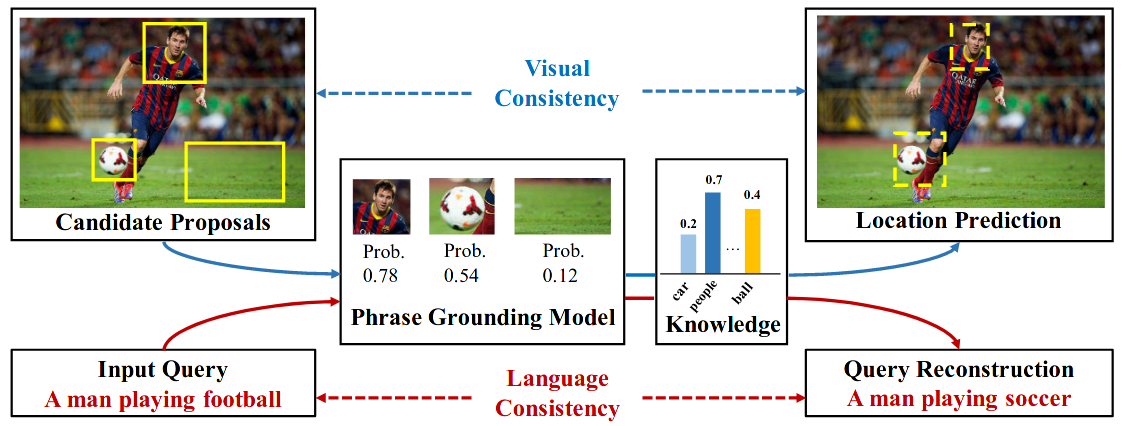
\includegraphics[width=.8\textwidth]{figures/kac-example.png}
  \caption[Knowledge Aided Consistency high-level architecture
  overview]{ Knowledge Aided Consistency high-level architecture
  overview \cite{chen2018knowledge}. The model applies external
  knowledge to downweight unrelated proposals, while it learns to
  ground by means of both visual and language reconstruction loss. }
  \label{fig:kac-example}
\end{figure}

In \cite{liu2019adaptive}, X. Liu \etal{} proposed a reconstruction
network based on attention map and optimized for the task of REG
(Sec.~\ref{sec:visual-grounding}). They first extract subject,
location and context features for both language and visual modalities.
Language features are extracted by means of an attention mechanism
applied on the sentence encoded with a Bi-LSTM network. Visual subject
features are instead extracted from object detector convolutional
layers, along with the position of proposal relative to the image for
the location features and neighbors features for context features.
Through a reconstruction module they learn to ground by optimizing
the reconstruction with respect to sentence, attributes and hidden
features (subject, location and context). The language is
reconstructed based on attentive proposal features encoded by the
Bi-LSTM, while attributes, used to distinguish objects of same
category, are reconstructed from plain proposal features. The adaptive
reconstruction instead reconstruct attentive hidden features by
combining the contribution of subject, location and context features
from both visual and language modalities.

S. Datta \textit{et al.} in \cite{datta2019align2ground} proposed to
learn to ground by optimizing the model for the downstream task of
caption-to-image retrieval. Here, the assert is that learning
caption-to-image retrieval intrinsically means learning to ground,
i.e., the models learns to return the correct image given a caption if
and only if it has understood to ground the caption with the image.
Such change of paradigm allow them to exploit the weak supervision
that in the proxy task becomes full supervision. Their model, outlined
in Fig.~\ref{fig:align2ground-model}, follows three stages. Firstly,
it project both visual and textual features in a joint embedding space
by linear projection. Then, using a similarity function, it computes
the similarity between each phrase and each proposal. For each phrase,
the module returns a random proposal among top-k ($k = 3$) similar
proposals wrt the phrase. The intention here is to produce a list of
caption-conditioned RoIs. In the second step, the model build a global
representation of previously matched RoIs with an order-invariant deep
encoder. The encoder is implemented as a two-layer MLP. Finally, the
model measure the similarity between the proposed image representation
and the query caption by first embeddings the caption $c$, encoded by
$\Phi_{RNN}$, in the same output space as the image representation
$I^c_{rois}$ by using a two-layer MLP $f_{enc}$:
\begin{equation}
  \hat{\bm{c}} = MLP (\Phi_{RNN} (c)) \qquad \hat{\bm{r}}_c = f_{enc} (I^c_{rois}).
\end{equation}
Then, it computes cosine similarity between the two multimodal
representations:
\begin{equation}
  S_{Ic} = \frac{ \hat{\bm{c}}^T \hat{\bm{r}}_c }{ || \hat{\bm{c}} ||_2 || \hat{\bm{r}}_c ||_2 }.
\end{equation}
where $S_{Ic}$ is the similarity between image $I$ and caption $c$. 

\begin{figure}
  \centering
  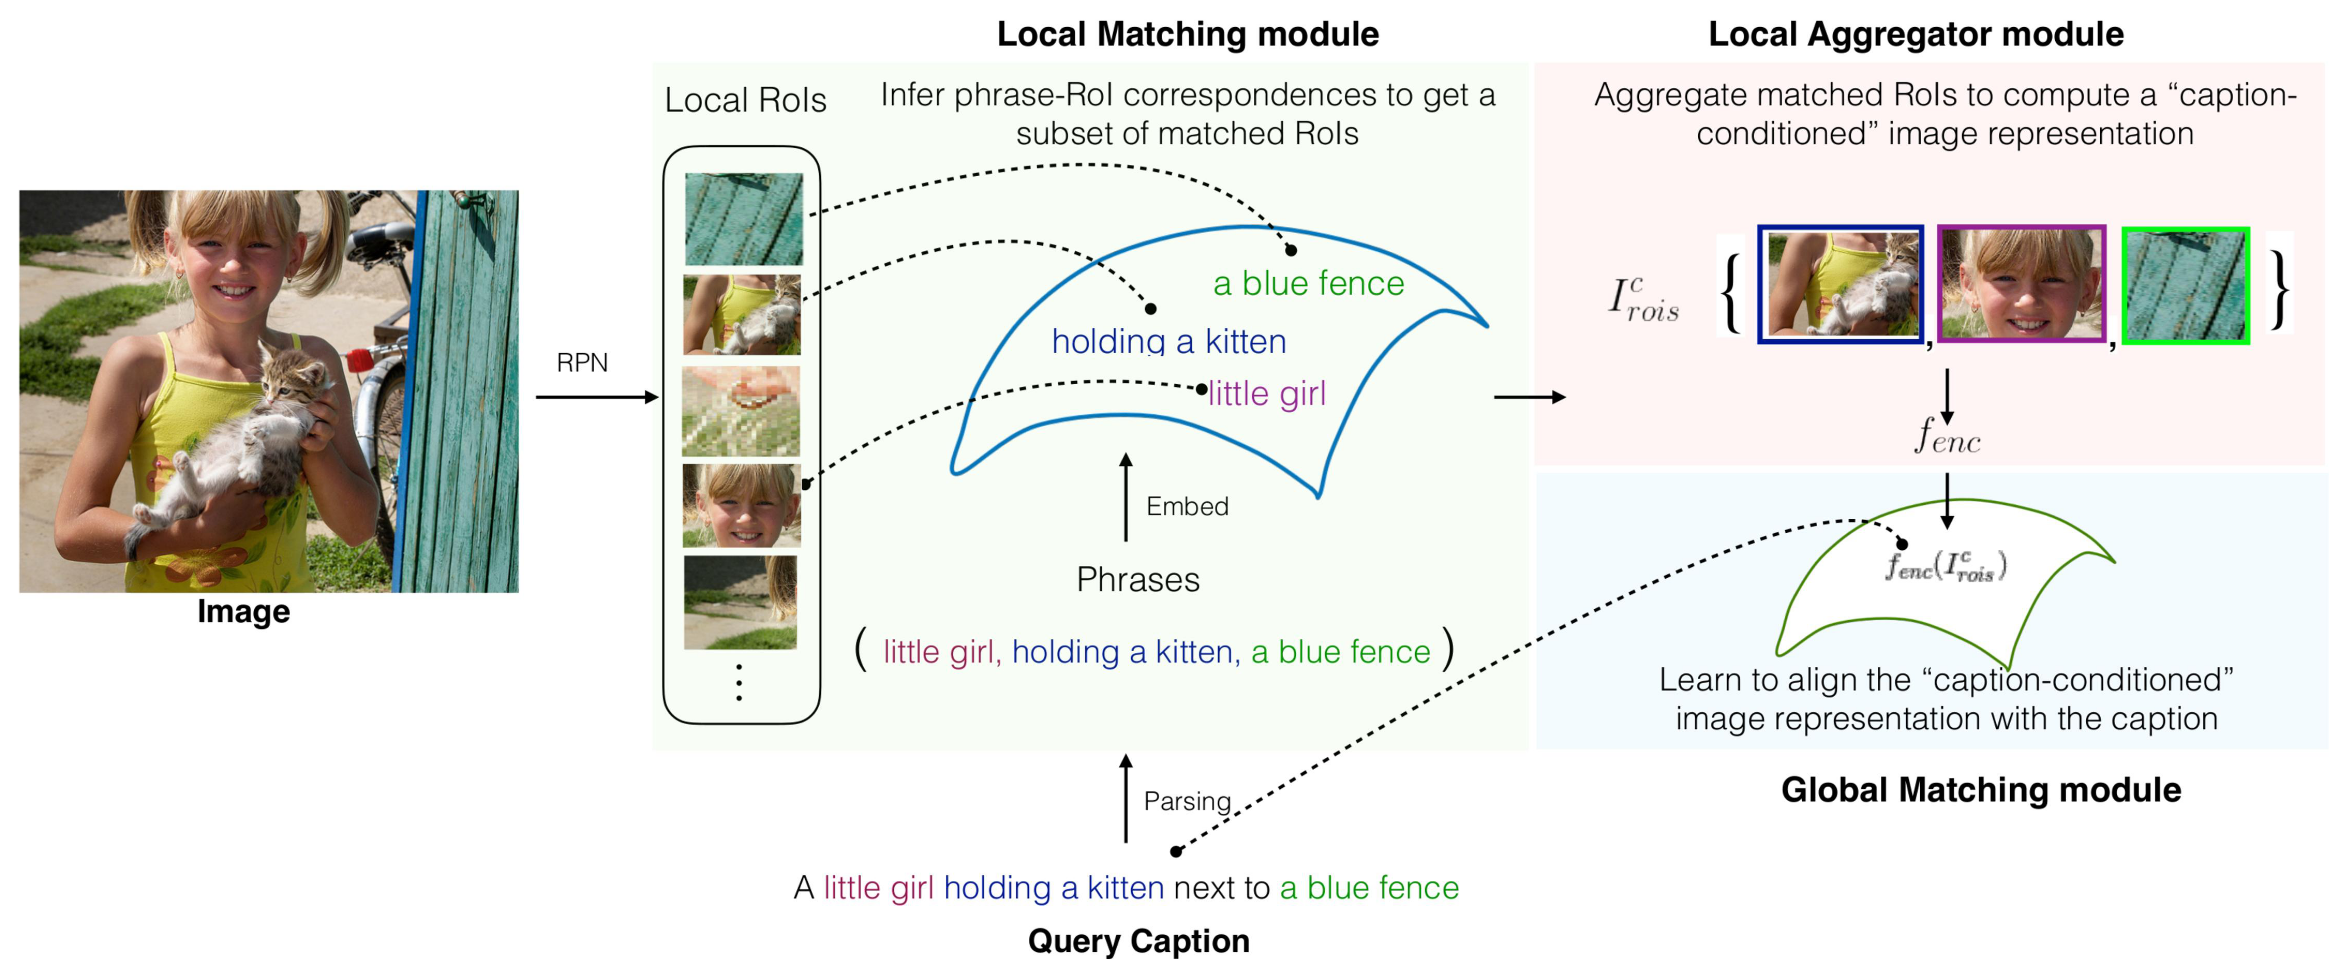
\includegraphics[width=.8\textwidth]{figures/align2ground-model.png}
  \caption[Align2Ground model overview]{Align2Ground model overview
  \cite{datta2019align2ground}. The query is parsed into chunks that
  are matched with image proposals by means of a similarity score
  computed between chunks and proposals the latent space. Matched
  regions are then fed into the order-invariant deep encoder which
  encodes this list of caption conditioned proposals. The global
  matching module measures the similarity between the global image
  representation made by caption-conditioned proposals and the input
  query and align image-caption pairs.}
  \label{fig:align2ground-model}
\end{figure}

An important contribution in phrase grounding comes from the work of
J. Wang in \etal{} in \cite{wang2019phrase}. Their approach is very
different wrt other works because it operates with no supervision. In
contrast to other works which usually leverage strong supervision or
weak supervision to learn mappings from phrase-image regions or pairs,
they do not use ground truth. Their approach is motivated by the
following assertion: ``We argue that such a non-paired setting better
reflects how humans localize objects in images -- not by memorizing
paired examples, but by assembling prior knowledge from more general
sources and tasks (e.g. recognizing concepts or attributes) to tackle
a more specialized task (phrase localization)''. Their model is built
on three steps, as Fig.~\ref{fig:phraseloc-model} shows. In the first
stage, they employ many object detectors (tfcoco, tfcoco2, places365,
yolo9000, colour) that vary in number and type of categories covered,
training data and accuracy in order to exploit their variance and
redundancy to retrieve information on objects in images. The second
stage computes the semantic similarity between each phrase and the
detector concept labels. Here, the underlying idea is that an object
in the image is more likely to be the target object when the concept
expressed in a phrase is similar to the concept expressed by the
proposal, or better, by its class label. Similarly to
\cite{chen2018knowledge}, they represent queries $q$ and labels $c$ as
$300$-dimensional CBOW word2vec embeddings. The goal of this stage is
to compute a ranked list of candidate bounding box detections based on
their similarity to the aggregate query phrase. Such list is extracted
by computing a similarity function $S(q, c)$ in the word embedding
space between the aggregate embedding of a query and the embedding of
a label. Here, a strong assumption is made: the similarity between
word embeddings perfectly captures the semantic similarity between
words, i.e, between representative word in phrase and label. The
representative word in phrase can be computed either by summing the
word vectors and normalizing to the unit vector (w2v-avg), or by
expressing each word separately (w2v) and utilizing just one of the
words for localization (w2v). In the latter case, the candidate could
be the last word in the phrase (w2v-last). However, this heuristic
highly depends on some assumption on data (e.g., the language).
Another heuristic instead consider the word with the highest semantic
similarity to any detected concepts (w2v-max). The third and last
stage localizes the bounding box given the ranked list of candidates.
At this point, given the target concept, the model only needs to
disambiguate between the group of proposal with the same concept, if
any. In this case they either
\begin{enumerate*}[label=(\roman*)] 
  \item select a random instance;
  \item select the instance with the largest bounding box; 
  \item select the instance with the highest class prediction
  confidence;
  \item generate a minimal bounding box enclosing all instances
  (union); and
  \item use a consensus strategy from detectors.
\end{enumerate*} 
The consensus strategy is slightly different wrt the other heuristics.
In this case they select top-k ($k = 5$) concepts and generates an
heatmap which reflect the votes from object detectors. The heatmap is
generated by heating up proposal that represent more concepts. The
hottest proposal is chosen. Even the proposed approach is very
promising it is not exempt from problems. First of all it requires
many object detectors to run, which in some case may be unfeasible.
Secondly, it uses heuristics designed on purpose for data, which, even
if very effective, hardly scale to other human languages or
differently collected corpus. This effect can be seen looking at the
unbalanced performance obtained on Flickr30k Entities (nearly 50\%
accuracy) which contains good quality phrases, compared to ReferIt
(nearly 26\% accuracy) that instead contains imprecise or erroneous
queries. (For more on both dataset see Sec.~\ref{sec:datasets}). 

\begin{figure}
  \centering
  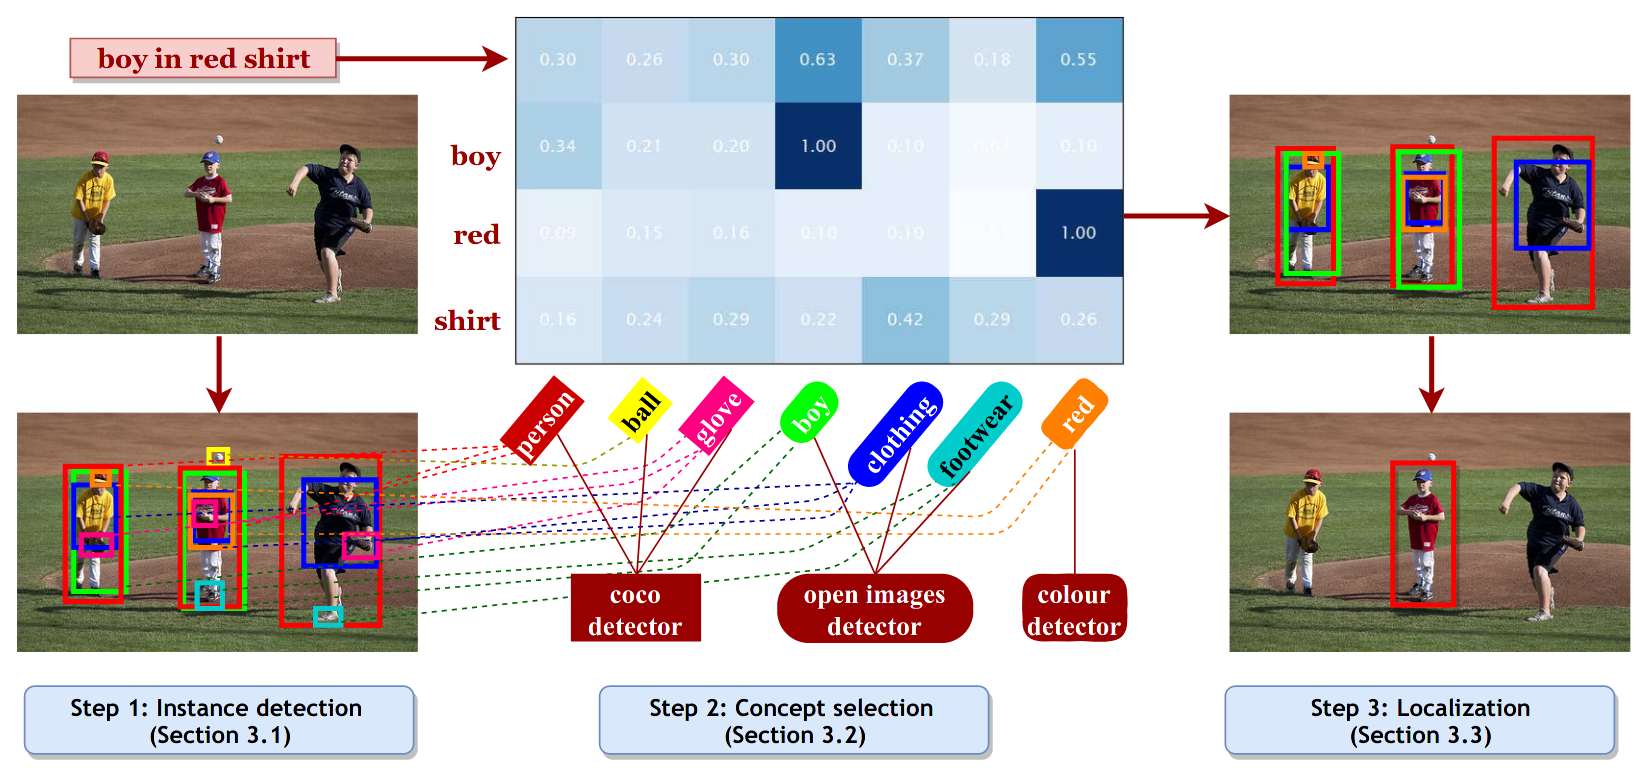
\includegraphics[width=.8\textwidth]{figures/phraseloc-model.png}
  \caption[Phrase Localization without Paired Training Examples model
  overview]{Phrase Localization without Paired Training Examples model
  overview \cite{wang2019phrase}. The first stage is responsible to
  retrieve information from proposals (class labels) and from text
  (concept). The second stage select a concept, among the other, that
  best matches proposals and query. The third stage localize a
  bounding box given the detected concept in previous stage.}
  \label{fig:phraseloc-model}
\end{figure}

T. Gupta \etal{} in \cite{gupta2020contrastive} proposed that learns
phrase grounding through contrastive learning. In particular, their
loss optimizes the model to learn a compatibility function by means of
an attention map. The compatibility function is enforced to be higher
on positive query and image (i.e., from the same example), while lower
or other (negative) images and queries. Negative queries are build
with a language model that substitutes noun words in true caption like
``Chocolate donut in front of a computer'' with contextually plausible
but untrue words like ``cookie''.

Q. Wang \etal{} in \cite{wang2020maf} proposed a multimodal alignment
framework (MAF), outlined in Fig.~\ref{fig:maf-model} that joins the
contrastive learning exploiting weakly-supervised annotations and the
power of external knowledge from pretrained object detector. Inspired
by \cite{wang2019phrase} which encompasses many heterogeneous
categories, they employ the Faster-R CNN
(Sec.~\ref{subsec:faster-rcnn}) object detector trained on $1600$
classes and $400$ attributes. Using a linear projection, they join
proposal features with the word embedding of proposal class label and
proposal attribute label, yielding $\bm{v}_m$. For the textual part,
they embed phrase $\bm{p}_n$ through word embeddings yielding
$\bm{h}_n,k$ and then, foreach $k$-th word in phrase and foreach $n$-th
phrase, they compute a score $\bm{a}^m_{n,k}$ representing the
similarity between such word $\bm{h}_{n,k}$ and proposal features
representation $\bm{v}_m$. The final attention score is the maximum
similarity between proposal features representation and word features
representation. Such attention is the normalized with softmax function
and used as weight for averaging words representation in phrase. A
projection matrix construct the final representation $\bm{e}_n$ for
phrases $p_n$. The model is optimized by a contrastive loss $\calL$
that aims to learn the visual and textual features by maximizing the
similarity score between paired image-caption elements and minimizing
the score between the negative samples:
\begin{equation}
  \calL = - \log \frac{e^{sim(I, S)}}{ \sum_{I' \in batch} e^sim(I', S) },
\end{equation}
where $sim(I, S)$ is the similarity function between image and query
sentence defined as:
\begin{equation}
  sim(I, S) = \frac{1}{N} \sum_n \max_m A_{n,m},
\end{equation}
where $A \in \Rset^{N \times M}$ is the phrase-object similarity
matrix, and its component is computed as:
\begin{equation}
  A_{n,m} = \bm{e}^T_n \bm{v}_m.
\end{equation}
Particularly, for each caption sentence, they use all the images $I′$
in the current batch as candidate (negative) examples.

\begin{figure}
  \centering
  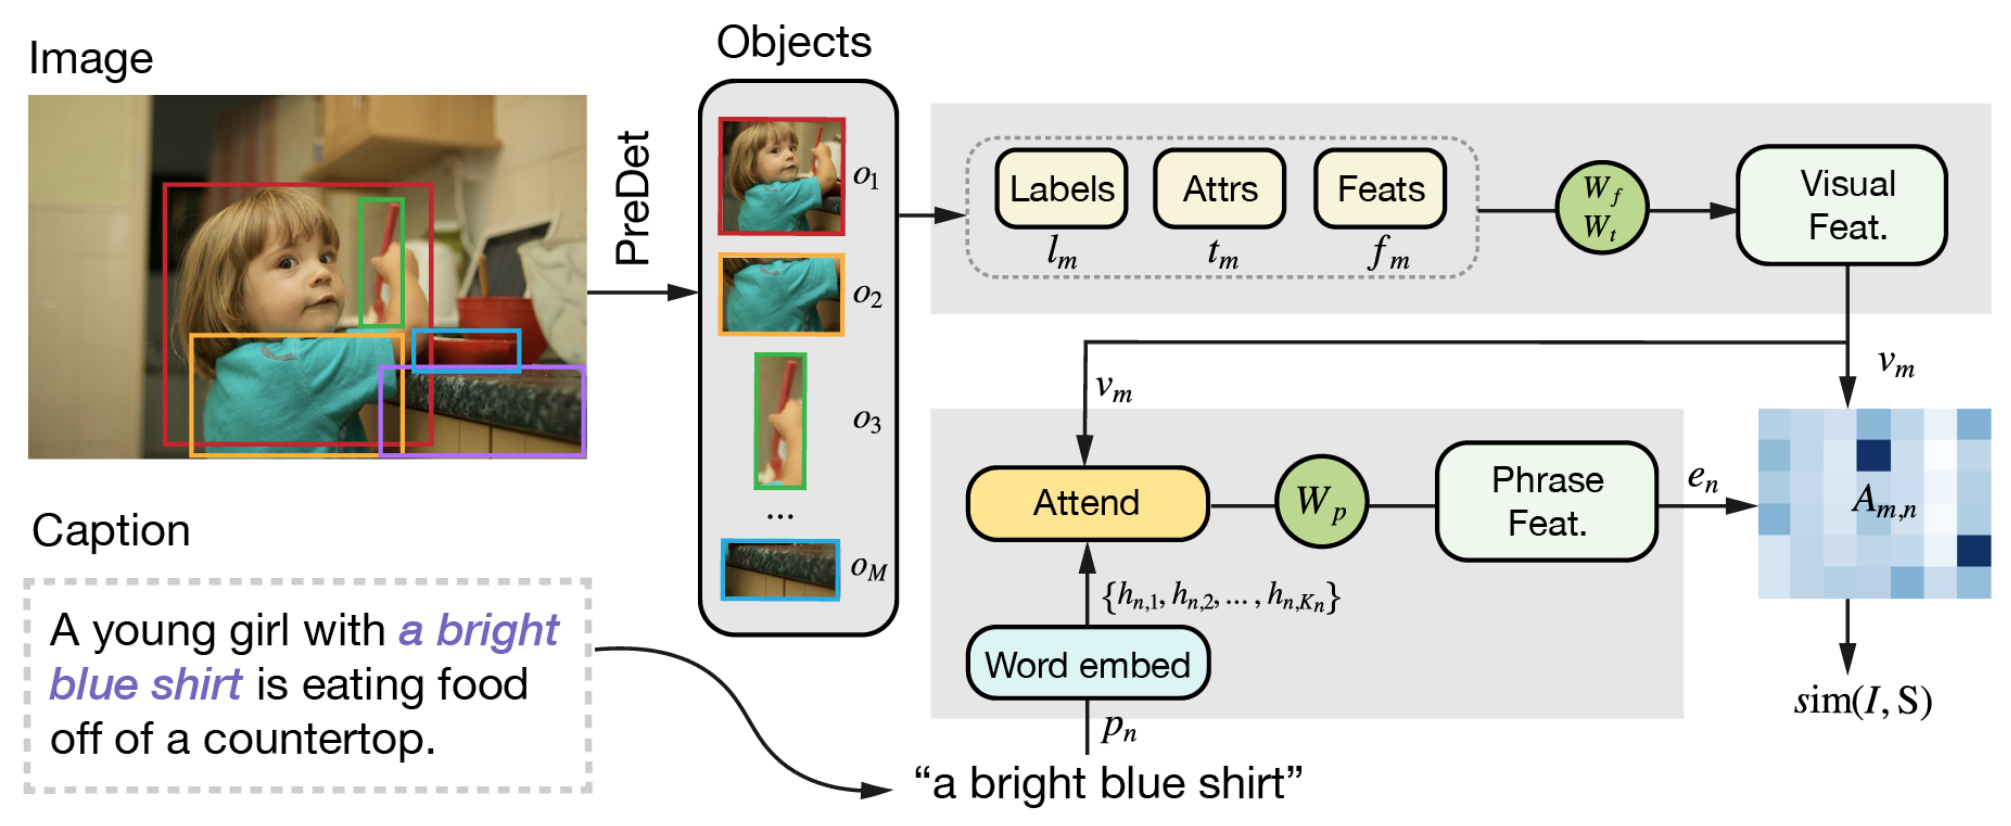
\includegraphics[width=.8\textwidth]{figures/maf-model.png}
  \caption[Multimodal Alignment Framework model overview]{Overview
  of our proposed Multimodal Alignment Framework (MAF)
  \cite{wang2020maf}. A dataset of images and their captions is the
  input to our model. PreDet predicts bounding boxes for objects in
  the image and their labels, attributes, and features, which are
  then integrated into visual feature representations. Attention is
  applied between word embedding and visual representations to
  compute the visually-aware language representations for phrases.
  Finally, a multi-modal similarity function is used to measure the
  caption-image relevance based on the phrase-object similarity
  matrix.}
  \label{fig:maf-model}
\end{figure}

\subsection{Supervised Works}

In terms of quantitative evaluation, models developed under supervised
settings show a strong boost in performance: in such environment, the
information of which is the bounding box that grounds the query is
available. Z. Yang \etal{} in \cite{yang2019fast} designed a novel
one-stage model (Sec.~\ref{sec:two-stage-vs-one-stage}), whose goal is
to outperform existing two-stage methods and overcome the problem of
the quality of the region candidates. ``if none of the candidates
could cover the ground truth region'', they argue, ``there is no hope
in the second stage to rank the right region to the top''. For this
reason, they propose a one-stage model that allows end-to-end joint
optimization. The main idea is to fuse text query's embedding into the
YOLOv3 object detector (Sec.~\ref{subsec:yolo}), along with spacial
features. In \cite{sadhu2019zero}, A. Sadhu \etal{} on the same line
of \cite{yang2019fast} proposed a one-stage model focusing on the
slightly different task of Zero Shot Grounding, which can include
unseen nouns in phrases. They argue that a two-stage approach
(Sec.~\ref{sec:two-stage-vs-one-stage}) is an obstacle due to the
constrained generation of appropriate proposals. Instead, they propose
a single-stage model which combines the detector network and the
grounding system and predicts classification scores and regression
parameters. A completely different approach is adopted by H. Zhang
\etal{} in \cite{zhang2018grounding} where, based on the variational
Bayesian method, they capturers context's information by exploiting
reciprocal relation between the referent and context. D. Rigoni
\etal{} in \cite{rigoni2021better} proposed a novel loss for the
problem of phrase grounding. They show that, although using a simple
multi-modal feature fusion component, their model is able to reach
good performance. Such loss employs metrics like Intersection Over
Union (IoU) and Complete IoU (CIoU).

\section{Visual Textual Knowledge Entity Linking}

Visual Textual Knowledge Entity Linking (VTKEL) introduced by S. Dost
\etal{} in \cite{dost2020jointly, dost2020vtkel, dost2020visual}, is
the task of grounding entities in image, text and knowledge, hence is
a more complex task than phrase localization. The introduction of
prior knowledge may enable semantic reasoning, and thus, being able to
solve VTKEL problem may lead to better understanding of semantic
information contained in the image and textual sentence, ending in a
better solution also for phrase grounding. However, due to the
complexity of the task (and its recent introduction) there are still
few works. 

\section{Visual Question Answering}

Visual Question Answering (VQA) is a computer vision task where a
system must infer the answer given a natural language question about
an image \cite{kafle2017visual}. VQA is a challenging task because it
encompasses many computer vision task, such us, object recognition or
detection, attribute or scene classification, counting and so on.
Moreover, questions are arbitrary, for example questions about spatial
relationships among objects or common sense reasoning may be asked.
Thus, solving the VQA task means being able to solve the phrase
localization task.

In \cite{kafle2017visual} authors made an awesome work collecting all
VQA related stuff:a proper definition of the problem, challenges,
motivations, datasets, metrics, algorithms and a summary of actual
main baseline models. As they highlight, among the large number of
algorithm proposed in literature, all consists of
\begin{enumerate*}[label=(\roman*)] 
  \item extracting image features,
  \item extracting question features, and
  \item producing an answer by combining these features.
\end{enumerate*}
VQA is mostly treated as a classification problem, where image and
question features are the input to the classification system, while
each unique answer is treated as a distinct category. The main
difference among existing systems is how they combine image and
question features. Some works uses simple combination mechanisms,
e.g., elementwise addition or multiplication, concatenation, while
others combine features using neural networks with bilinear pooling or
similar schemes. Other approaches consists in computing spatial
attention maps based on question features for focusing on visual
features, eventually, local features may also be scaled based on
importance. A few works use Bayesian models that exploit relationship
between question, image and answer distribution. Others instead break
VQA task into a series of sub-problems.
